\subsection{Experimental setup}
\label{sec:setup}

\subsubsection{System}
\label{sec:system}

In our experiments, we employ a server equipped with an x86-based 64-bit AMD EPYC-7742 processor. It operates at\ignore{a clock frequency of} $2.25$ GHz and is paired with $512$ GB of DDR4 system memory. Each core features a $4$ MB L1 cache, a $32$ MB L2 cache, and a shared L3 cache of $256$ MB. The server runs on Ubuntu 20.04.


\subsubsection{Configuration}
\label{sec:configuration}

We utilize a 32-bit unsigned integer format for vertex IDs and 32-bit floating-point representation for edge weights. However, for\ignore{hashtable values,} total edge weight calculations, modularity computation, and any instances requiring aggregation or summation of floating-point values, we employ the 64-bit floating-point format. Affected vertices and changed communities are denoted by 8-bit integer vectors. In computing the weighted degree of each vertex, the local moving phase, the refinement phase, and aggregating edges for the super-vertex graph, we leverage OpenMP's \textit{dynamic schedule} with a chunk size of $2048$ to facilitate dynamic workload balancing among threads. However, for the aggregation phase of ND, DS, and DF Leiden, we use a chunk size of $32$ instead, as discussed in Section \ref{sec:approach}. Key parameters are configured as follows: the iteration tolerance $\tau$ is set to $10^{-2}$, the tolerance drop per pass $TOLERANCE\_DECLINE\_FACTOR$ to $10$ (as part of threshold-scaling optimization), the maximum number of iterations per pass $MAX\_ITERATIONS$ to $20$, and the maximum number of passes $MAX\_PASSES$ to $10$. Unless explicitly specified, all parallel implementations are executed with a default of $64$ threads, matching the available number of cores on the system. Compilation is carried out using GCC 9.4 and OpenMP 5.0 \cite{openmp18}.


\subsubsection{Dataset}
\label{sec:dataset}

To conduct experiments on large static graphs with random batch updates, we employ $12$ graphs listed in Table \ref{tab:dataset-large}, obtained from the SuiteSparse Matrix Collection \cite{suite19}. For these graphs, the number of vertices range from $3.07$ to $214$ million, and the number of edges range from $25.4$ million to $3.80$ billion.\ignore{With each graph, we ensure that all edges are undirected and weighted, with a default weight of $1$.} For experiments involving real-world dynamic graphs, we utilize five temporal networks sourced from the Stanford Large Network Dataset Collection \cite{snapnets}, detailed in Table \ref{tab:dataset}. Here, the number of vertices span from $24.8$ thousand to $2.60$ million, temporal edges from $507$ thousand to $63.4$ million, and static edges from $240$ thousand to $36.2$ million. With each graph, we ensure that all edges are undirected and weighted, with a default weight of $1$.

\begin{table}[hbtp]
  \centering
  \caption{List of $12$ graphs retrieved from the SuiteSparse Matrix Collection \cite{suite19} (with directed graphs indicated by $*$). Here, $|V|$ denotes the number of vertices, $|E|$ denotes the number of edges (after making the graph undirected by adding reverse edges), and $|\Gamma|$ denotes the number of communities obtained with \textit{Static Leiden} algorithm \cite{sahu2023gveleiden}.}
  \label{tab:dataset-large}
  \begin{tabular}{|c||c|c|c|}
    \toprule
    \textbf{Graph} &
    \textbf{\textbf{$|V|$}} &
    \textbf{\textbf{$|E|$}} &
    \textbf{\textbf{$|\Gamma|$}} \\
    \midrule
    \multicolumn{4}{|c|}{\textbf{Web Graphs (LAW)}} \\ \hline
    indochina-2004$^*$ & 7.41M & 341M & 2.68K \\ \hline
    arabic-2005$^*$ & 22.7M & 1.21B & 2.92K \\ \hline
    uk-2005$^*$ & 39.5M & 1.73B & 18.2K \\ \hline
    webbase-2001$^*$ & 118M & 1.89B & 2.94M \\ \hline
    it-2004$^*$ & 41.3M & 2.19B & 4.05K \\ \hline
    sk-2005$^*$ & 50.6M & 3.80B & 2.67K \\ \hline
    \multicolumn{4}{|c|}{\textbf{Social Networks (SNAP)}} \\ \hline
    com-LiveJournal & 4.00M & 69.4M & 3.09K \\ \hline
    com-Orkut & 3.07M & 234M & 36 \\ \hline
    \multicolumn{4}{|c|}{\textbf{Road Networks (DIMACS10)}} \\ \hline
    asia\_osm & 12.0M & 25.4M & 2.70K \\ \hline
    europe\_osm & 50.9M & 108M & 6.13K \\ \hline
    \multicolumn{4}{|c|}{\textbf{Protein k-mer Graphs (GenBank)}} \\ \hline
    kmer\_A2a & 171M & 361M & 21.1K \\ \hline
    kmer\_V1r & 214M & 465M & 10.5K \\ \hline
  \bottomrule
  \end{tabular}
\end{table}

\begin{table}[hbtp]
  \centering
  \caption{List of $5$ real-world dynamic graphs\ignore{, i.e., temporal networks}, sourced from the Stanford Large Network Dataset Collection \cite{snapnets}. Here, $|V|$ denotes the number of vertices, $|E_T|$ represents the count of temporal edges (inclusive of duplicates), and $|E|$ indicates the number of static edges (without duplicates).}
  \label{tab:dataset}
  \begin{tabular}{|c||c|c|c|c|}
    \toprule
    \textbf{Graph} &
    \textbf{\textbf{$|V|$}} &
    \textbf{\textbf{$|E_T|$}} &
    \textbf{\textbf{$|E|$}} \\
    \midrule
    sx-mathoverflow & 24.8K & 507K & 240K \\ \hline
    sx-askubuntu & 159K & 964K & 597K \\ \hline
    sx-superuser & 194K & 1.44M & 925K \\ \hline
    wiki-talk-temporal & 1.14M & 7.83M & 3.31M \\ \hline
    sx-stackoverflow & 2.60M & 63.4M & 36.2M \\ \hline
  \bottomrule
  \end{tabular}
\end{table}



\subsubsection{Batch generation}
\label{sec:batch-generation}

For experiments on large graphs with random batch updates, we take each base graph from Table \ref{tab:dataset-large} and generate random batch updates \cite{com-zarayeneh21}, comprising an $80\% : 20\%$ mix of edge insertions and deletions to emulate realistic batch updates, with each edge having a weight of $1$. To prepare the set of edges for insertion, we select vertex pairs with equal probability. For edge deletions, we uniformly delete existing edges. To simplify, no new vertices are added or removed from the graph. The batch size is measured as a fraction of the edges in the original graph, ranging from $10^{-7}$ to $0.1$ (i.e., $10^{-7}|E|$ to $0.1|E|$). Multiple batches are generated for each size to allow averaging.\ignore{For a billion-edge graph, this translates to a batch size ranging from $100$ to $100$ million edges.} All batch updates are undirected, meaning for every edge insertion $(i, j, w)$ in the batch update, the edge $(j, i, w)$ is also included. We employ five distinct random batch updates for each batch size and report the average across these runs in our experiments. For experiments involving real-world dynamic graphs, we start by loading $90\%$ of each graph from Table \ref{tab:dataset}, and ensure all edges are weighted with a default weight of $1$ and are undirected by adding reverse edges. Subsequently, we load $B$ edges in $100$ batch updates. Here, $B$ denotes the desired batch size, specified as a fraction of the total number of temporal edges $|E_T|$ in the graph, and ensure the batch update is undirected.


\subsubsection{Measurement}
\label{sec:measurement}

We measure the runtime of each method on the entire updated graph, covering all stages: the local-moving phase, refinement phase, aggregation phase, initial and incremental marking of affected vertices, convergence detection, and any necessary intermediate steps.\ignore{Memory allocation and deallocation times are excluded.} We assume that the total edge weight of the graphs is known and can be tracked with each batch update. It is important to note that none of the algorithms discussed here, i.e., Static, ND, DS, and ND Leiden, produce communities that are internally disconnected, so we omit this from our figures. Additionally, our implementation of Static Leiden is significantly faster than existing implementations, as demonstrated in our report \cite{sahu2023gveleiden}.

\begin{figure*}[hbtp]
  \centering
  \subfigure[Overall result]{
    \label{fig:8020-runtime--mean}
    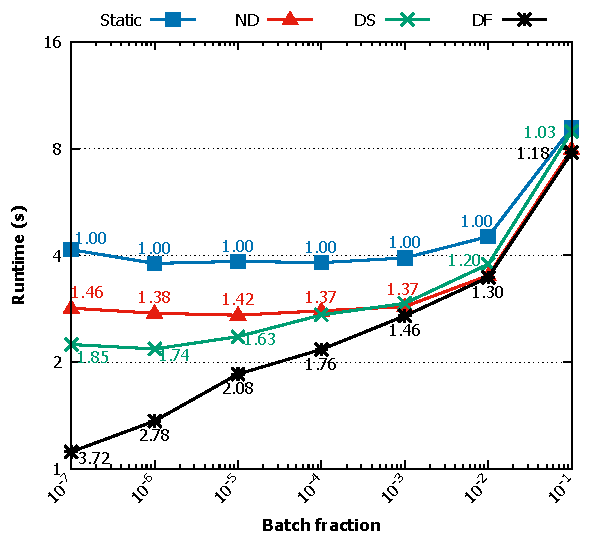
\includegraphics[width=0.38\linewidth]{out/8020-runtime-mean.pdf}
  }
  \subfigure[Results on each graph]{
    \label{fig:8020-runtime--all}
    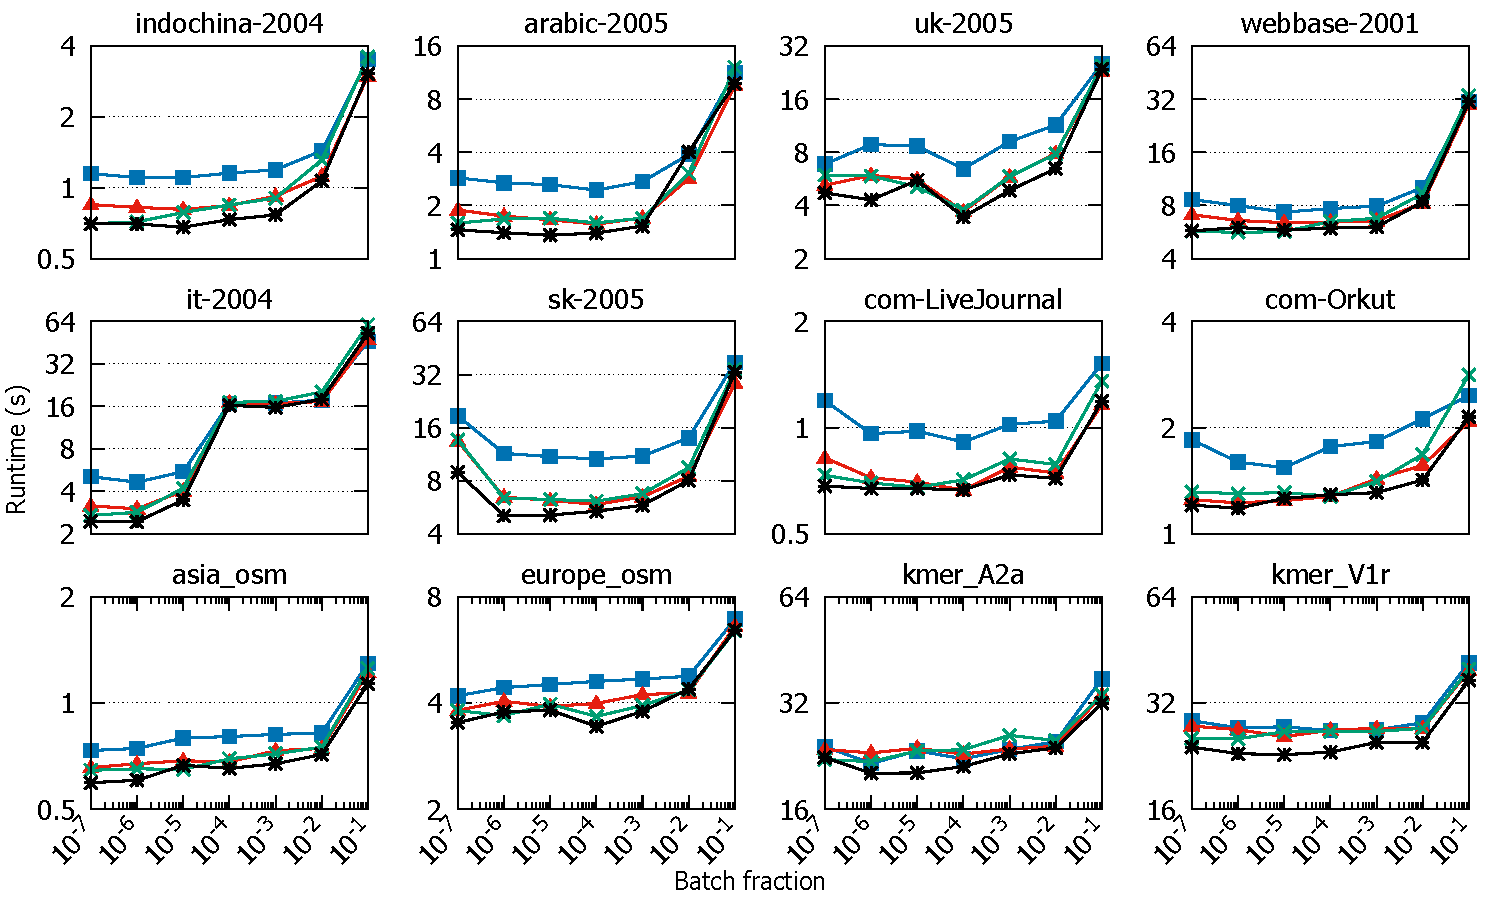
\includegraphics[width=0.58\linewidth]{out/8020-runtime-all.pdf}
  } \\[0ex]
  \caption{Runtime (logarithmic scale) of our multicore implementation of \textit{Naive-dynamic (ND)}, \textit{Delta-screening (DS)}, and \textit{Dynamic Frontier (DF) Leiden}, compared to \textit{Static Leiden} \cite{sahu2024fast}, on large\ignore{(static)} graphs with randomly generated batch updates. The size of these batch updates ranges from $10^{-7}|E|$ to $0.1|E|$ in multiples of $10$, with the updates comprising $80\%$ edge insertions and $20\%$ edge deletions to simulate realistic dynamic graph changes. The right subfigure shows the runtime of each algorithm for individual graphs in the dataset, while the left subfigure displays overall runtimes using the geometric mean for consistent scaling across graphs.\ignore{Furthermore,} The speedup of each algorithm compared to Static Leiden is indicated on the respective lines.}
  \label{fig:8020-runtime}
\end{figure*}

\begin{figure*}[hbtp]
  \centering
  \subfigure[Overall result]{
    \label{fig:8020-modularity--mean}
    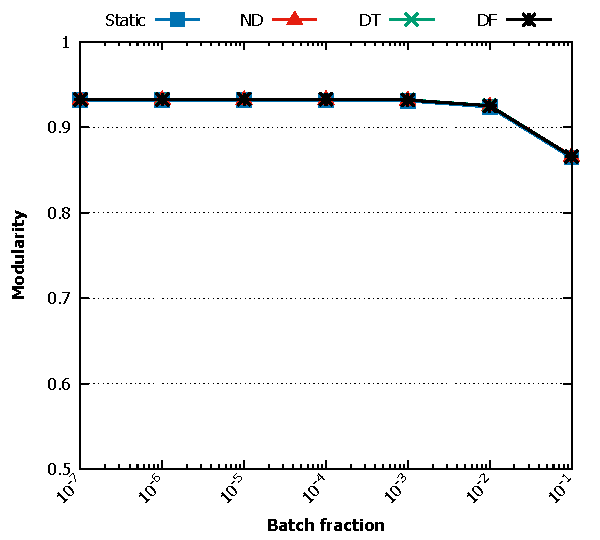
\includegraphics[width=0.38\linewidth]{out/8020-modularity-mean.pdf}
  }
  \subfigure[Results on each graph]{
    \label{fig:8020-modularity--all}
    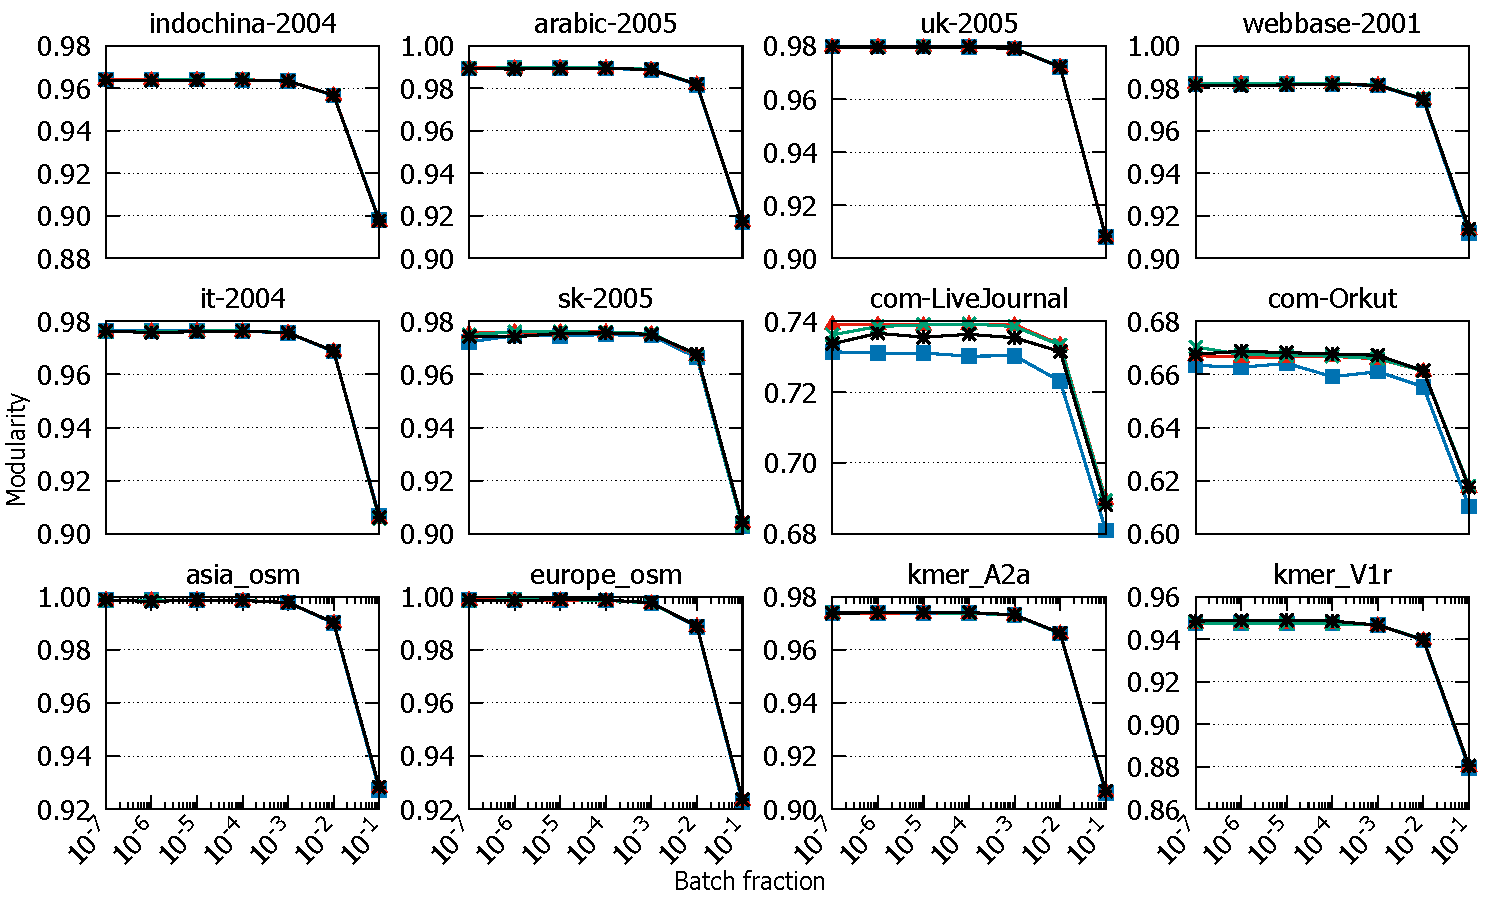
\includegraphics[width=0.58\linewidth]{out/8020-modularity-all.pdf}
  } \\[-2ex]
  \caption{Modularity comparison of our multicore implementation of \textit{Static}, \textit{Naive-dynamic (ND)}, \textit{Delta-screening (DS)}, and \textit{Dynamic Frontier (DF)} Leiden on large (static) graphs with generated random batch updates. The size of batch updates range from $10^{-7} |E|$ to $0.1 |E|$ in multiples of $10$ (logarithmic scale), consisting of $80\%$ edge insertions and $20\%$ edge deletions to simulate realistic dynamic graph updates. The right subfigure depicts the modularity for each approach in relation to each graph, while the left subfigure showcases overall modularity using arithmetic mean.}
  \label{fig:8020-modularity}
\end{figure*}

\begin{figure*}[!hbt]
  \centering
  \subfigure[Overall Runtime]{
    \label{fig:temporal-summary--runtime-overall}
    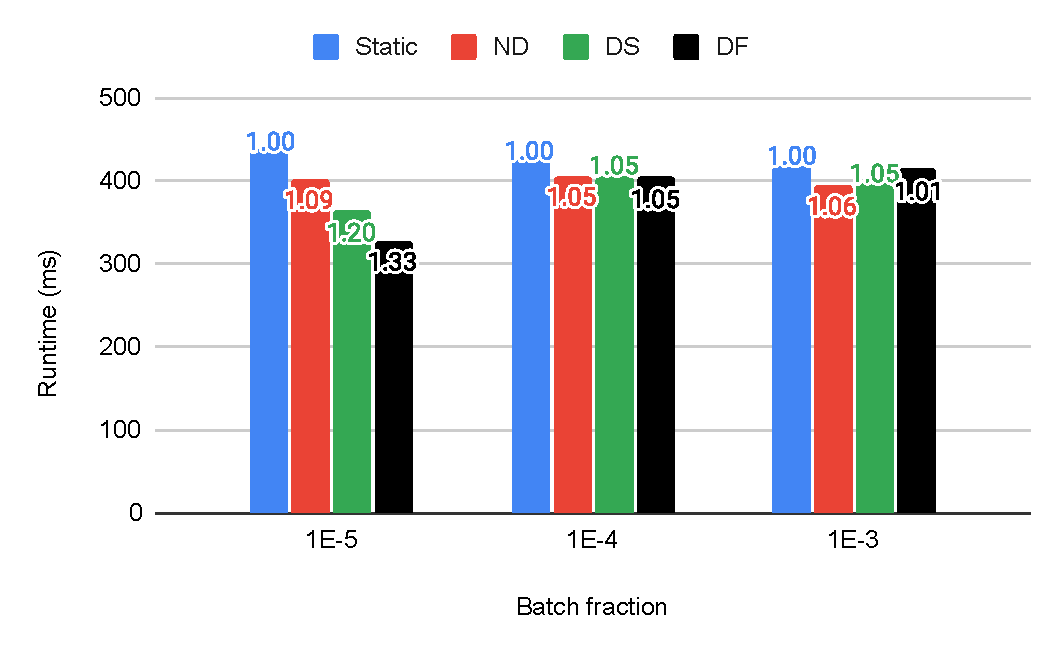
\includegraphics[width=0.48\linewidth]{out/temporal-summary-runtime-overall.pdf}
  }
  \subfigure[Overall Modularity of communities obtained]{
    \label{fig:temporal-summary--modularity-overall}
    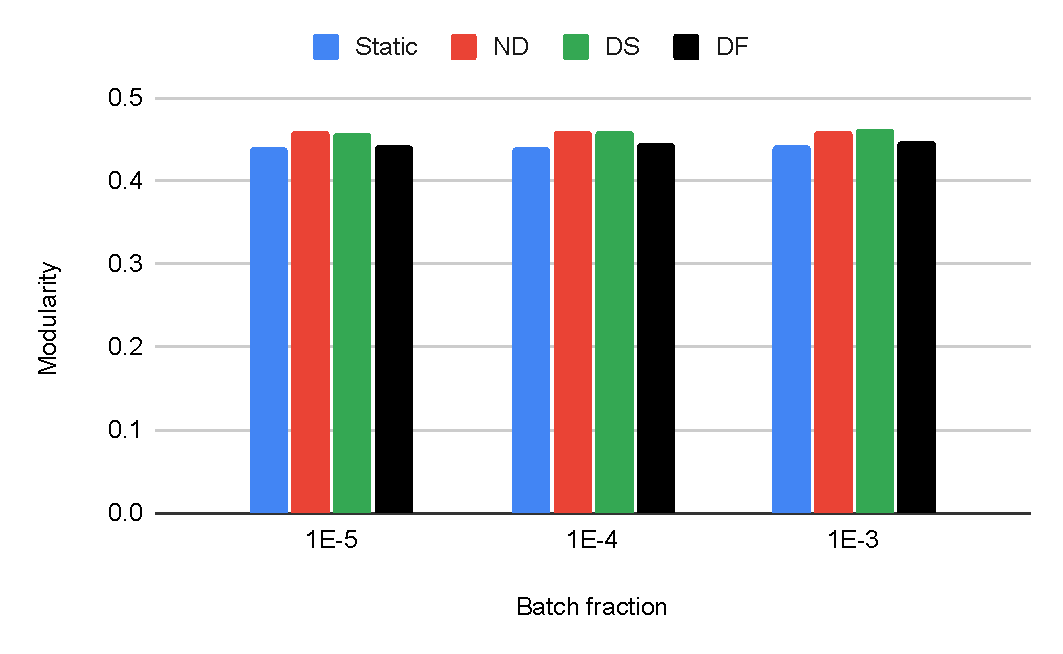
\includegraphics[width=0.48\linewidth]{out/temporal-summary-modularity-overall.pdf}
  } \\[2ex]
  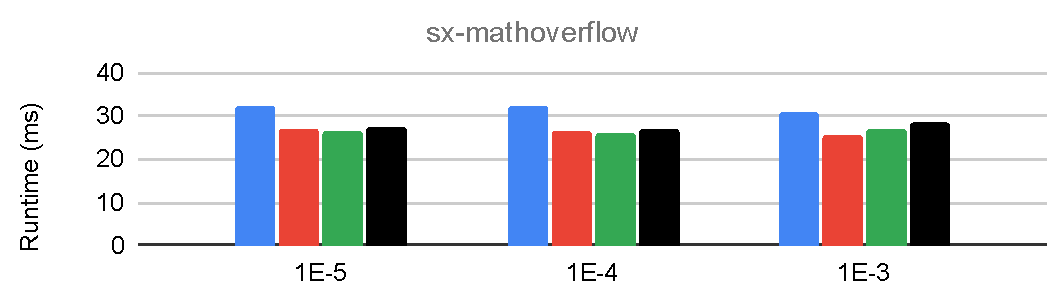
\includegraphics[width=0.48\linewidth]{out/temporal-summary-runtime-sx-mathoverflow.pdf}
  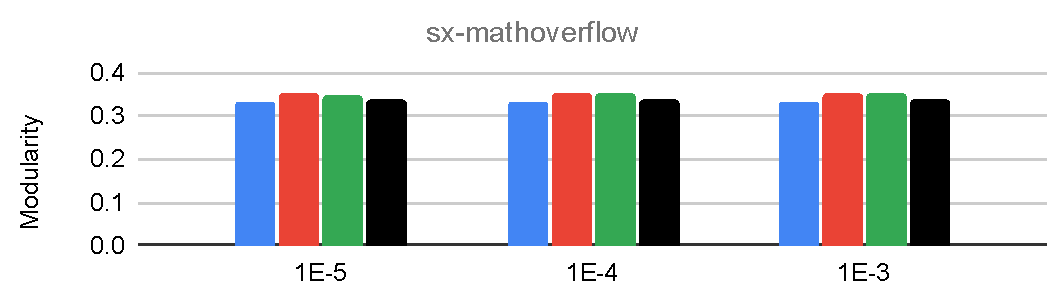
\includegraphics[width=0.48\linewidth]{out/temporal-summary-modularity-sx-mathoverflow.pdf}
  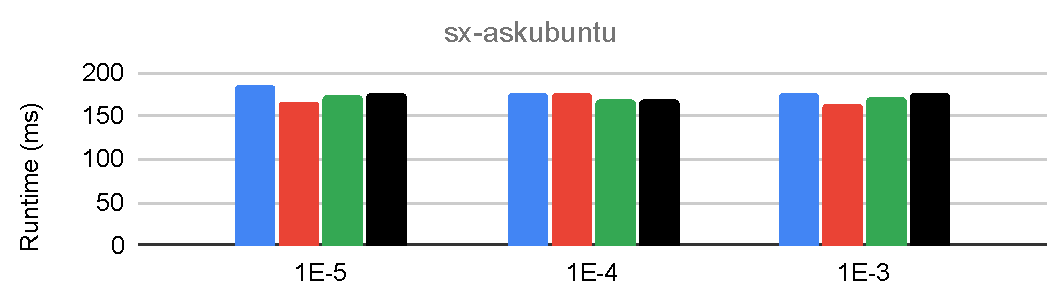
\includegraphics[width=0.48\linewidth]{out/temporal-summary-runtime-sx-askubuntu.pdf}
  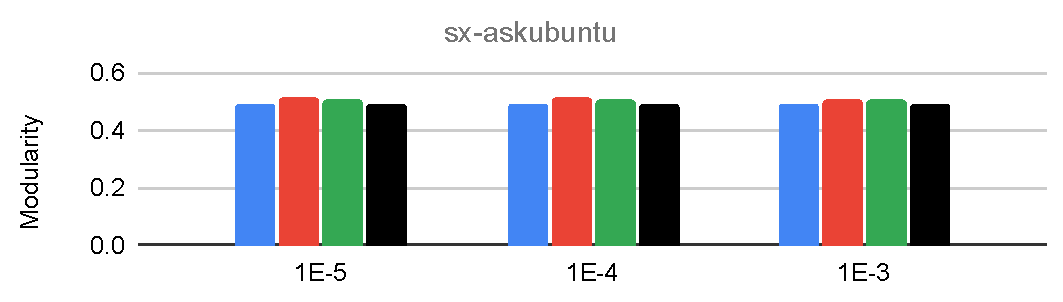
\includegraphics[width=0.48\linewidth]{out/temporal-summary-modularity-sx-askubuntu.pdf}
  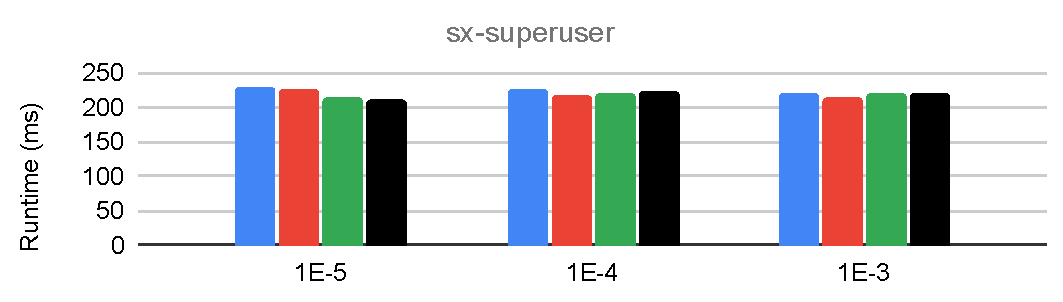
\includegraphics[width=0.48\linewidth]{out/temporal-summary-runtime-sx-superuser.pdf}
  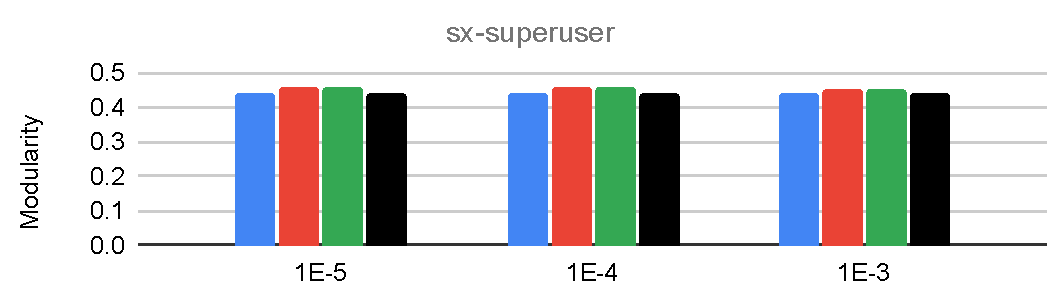
\includegraphics[width=0.48\linewidth]{out/temporal-summary-modularity-sx-superuser.pdf}
  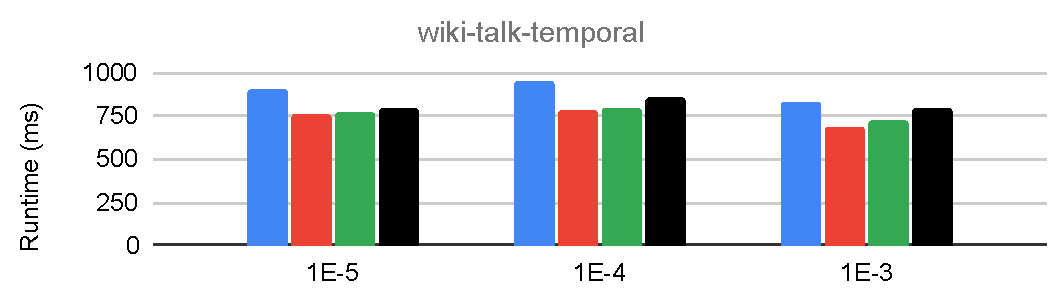
\includegraphics[width=0.48\linewidth]{out/temporal-summary-runtime-wiki-talk-temporal.pdf}
  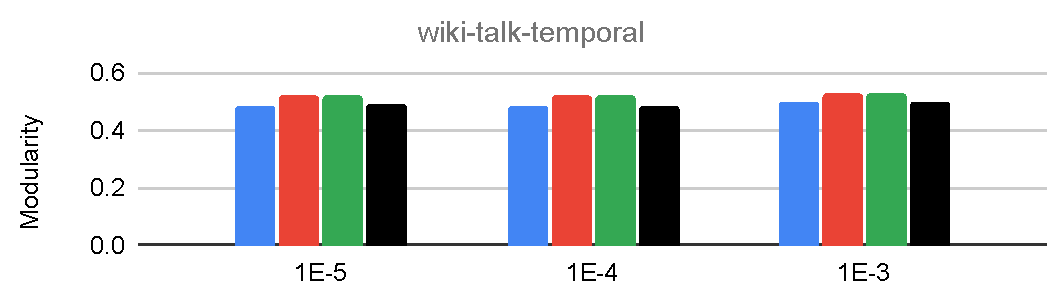
\includegraphics[width=0.48\linewidth]{out/temporal-summary-modularity-wiki-talk-temporal.pdf}
  \subfigure[Runtime on each dynamic graph]{
    \label{fig:temporal-summary--runtime-graph}
    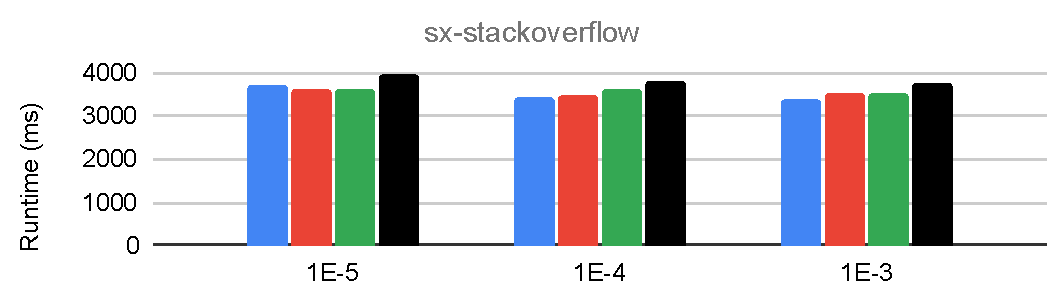
\includegraphics[width=0.48\linewidth]{out/temporal-summary-runtime-sx-stackoverflow.pdf}
  }
  \subfigure[Modularity in communities obtained on each dynamic graph]{
    \label{fig:temporal-summary--modularity-graph}
    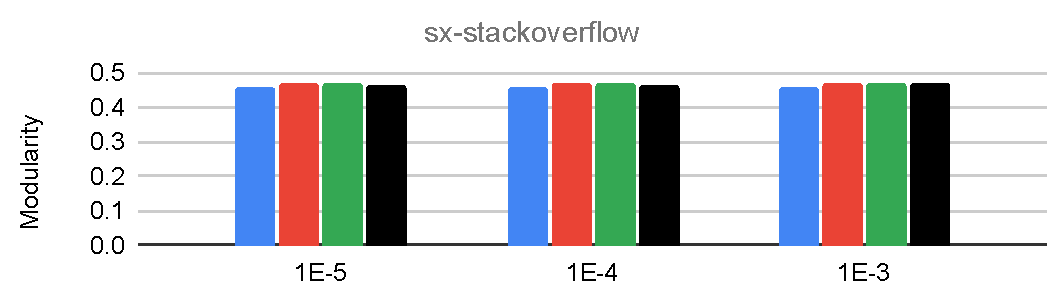
\includegraphics[width=0.48\linewidth]{out/temporal-summary-modularity-sx-stackoverflow.pdf}
  } \\[-2ex]
  \caption{Mean Runtime and Modularity of communities obtained with our multicore implementation of \textit{Static}, \textit{Naive-dynamic (ND)}, \textit{Delta-screening (DS)}, and \textit{Dynamic Frontier (DF)} Leiden on real-world dynamic graphs, with batch updates of size $10^{-5}|E_T|$ to $10^{-3}|E_T|$. Here, (a) and (b) show the overall runtime and modularity across all temporal graphs, while (c) and (d) show the runtime and modularity for each graph. In (a), the speedup of each approach with respect to Static Leiden is labeled.}
  \label{fig:temporal-summary}
\end{figure*}





\subsection{Performance Comparison}
\label{sec:performance-comparison}

\subsubsection{Results on large graphs with random batch updates}

We now evaluate the performance of our parallel implementations of Static, Naive-dynamic (ND), Delta-screening (DS), and Dynamic Frontier (DF) Leiden on large (static) graphs listed in Table \ref{tab:dataset-large}, using randomly generated batch updates. As detailed in Section \ref{sec:batch-generation}, the batch updates range in size from $10^{-7}|E|$ to $0.1|E|$ (in multiples of $10$), consisting of $80\%$ edge insertions and $20\%$ edge deletions to simulate realistic scenarios. Reverse edges are included with each batch update to maintain the graph as undirected. As stated in Section \ref{sec:batch-generation}, we generate $5$ different random batch updates for each batch size to reduce measurement noise. Figure \ref{fig:8020-runtime} presents the runtime of Static, ND, DS, and DF Leiden, while Figure \ref{fig:8020-modularity} shows the modularity of the communities obtained with each approach.

Figure \ref{fig:8020-runtime--mean} demonstrates that ND, DS, and DF Leiden achieve mean speedups of $1.37\times$, $1.47\times$, and $1.98\times$, respectively, when compared to Static Leiden. Let us now discuss why ND, DS, and DF Leiden exhibit only modest speedups over Static Leiden. Unlike Louvain algorithm, we must always run the refinement phase of Leiden algorithm to avoid badly connected and internally disconnected communities. Nonetheless, the refinement phase splits the communities obtained/updated from the local-moving phase into several smaller sub-communities. Stopping the passes early, as done with DF Louvain, leads to low modularity for ND/DS/DF Leiden because sufficiently large high-quality clusters have not yet formed due to the refinement phase. Further, ND/DS/DF Leiden can only reduce the runtime of the local-moving phase of the first pass of the Leiden algorithm. However, only about $37\%$ of the runtime in Static Leiden is spent in the local-moving phase of the first pass. These factors constrain the speedup potential of ND, DS, and DF Leiden over Static Leiden. It should also be noted that unlike Static Leiden, ND/DS/DF Leiden allow tracking of communities on dynamic graphs. Figures \ref{fig:8020-modularity--mean} and \ref{fig:8020-modularity--all} show that ND, DS, and DF Leiden achieve communities with approximately the same modularity as Static Leiden. Thus, for large graphs with random batch updates, DF Leiden appears to be the dynamic community detection method of choice for tracking evolving communities.

Also note in Figure \ref{fig:8020-runtime} that the runtime of Static Leiden increases with larger batch updates. This phenomenon can be attributed to the random batch updates, which indiscriminately disturb the original community structure, necessitating Static Leiden to undergo more iterations to converge, rather than solely due to the increased number of edges in the graph.


\subsubsection{Results on real-world dynamic graphs}

We also evaluate the performance of our parallel implementations of Static, ND, DS, and DF Leiden on real-world dynamic graphs listed in Table \ref{tab:dataset}. These evaluations are performed on batch updates ranging from $10^{-5}|E_T|$ to $10^{-3}|E_T|$ in multiples of $10$. For each batch size, as described in Section \ref{sec:batch-generation}, we load $90\%$ of the graph, add reverse edges to ensure all edges are undirected, and then load $B$ edges (where $B$ is the batch size) consecutively in $100$ batch updates. Figure \ref{fig:temporal-summary--runtime-overall} shows the overall runtime of each approach across all graphs for each batch size, while Figure \ref{fig:temporal-summary--modularity-overall} depicts the overall modularity of the obtained communities. Additionally, Figures \ref{fig:temporal-summary--runtime-graph} and \ref{fig:temporal-summary--modularity-graph} present the mean runtime and modularity of the communities obtained with each approach on individual dynamic graphs in the dataset.

Figure \ref{fig:temporal-summary--runtime-overall} illustrates that ND Leiden is, on average, $1.09\times$ faster than Static Leiden for batch updates ranging from $10^{-5}|E_T|$ to $10^{-3}|E_T|$. In comparison, DS and DF Leiden exhibit average speedups of $1.20\times$ and $1.33\times$, respectively, over Static Leiden for the same batch updates. We now explain why ND, DS, and DF Leiden achieve only minor speedups over Static Leiden. Our experiments indicate that only about $20\%$ of the overall runtime of Static Leiden is spent in the local-moving phase of the first pass.\ignore{This is a significant decrease from the $37\%$ observed on large graphs with random batch updates.} Consequently, the speedup achieved by ND, DS, and DF Leiden relative to Static Leiden is limited. Furthermore, our observations suggest that while DF Leiden can reduce the time spent in the local-moving phase slightly more than ND Leiden, it incurs increased runtimes in the refinement and aggregation phases of the algorithm. This is likely because ND Leiden is able to optimize clusters more effectively than DF Leiden, which accelerates the refinement and aggregation phases for ND Leiden, albeit by a small margin. This explains the lower speedup of DF Leiden compared to ND Leiden on larger batch updates\ignore{of real-world dynamic graphs}.\ignore{Therefore, we recommend ND Leiden for real-world dynamic graphs.}

% Unlike with large graphs and random batch updates, on real-world dynamic graphs, we disable the aggregation tolerance $\tau_{agg}$. This results in a reduced portion of runtime spent in the local-moving phase of the first pass, which is the phase that can be minimized by the dynamic approaches. Specifically, we observe that only about $20\%$ of the overall runtime of Static Leiden is spent in the local-moving phase of the first pass.